\chapter{Background}\label{ch:background}
The first section of this chapter, section~\ref{sec:terminology}, explains terms that are used throughout this thesis. The next section, Android development methods~\ref{sec:android-development-methods}, gives an overview of different methods of developing an Android mobile application. The following section, lines of code~\ref{sec:lines-of-code}, describes lines of code as a software metric and what it measures. Lastly, the section related work~\ref{sec:further-reading}, suggests further reading to this investigation. 

\section{Terminology}\label{sec:terminology}
\begin{description}
  \item[Development methods] \hfill \\
    Refers to the two development methods investigated in this paper. I.e. developing the mobile application using the PhoneGap framework and with the Android framework using the Android SDK
  \item[Native function] \hfill \\
     A hardware function of a device, such as the accelerometer. A native function is implemented by the device's operating system and can be called by the software of the device.     
  \item[Web/Mobile application layer] \hfill \\
	Refers in the context of this paper to the application layer belonging specifically to the mobile application or the web application. The client side of a web application is run within a browser engine, usually a web browser such as Google Chrome or Internet Explorer. The client side of a web application can also be run in other browser enginges, in Android there is a browser engine called WebView. An Android mobile application can run the client side of a web application in a WebView, which then is a part of the mobile application. To be able to refer to the logic of the web application's client side that is run in the mobile application, the term web application layer is used. To term mobile application layer is used to refer to the logic of the mobile application excluding the web application layer.
	\item[Native application] \hfill \\
	A native application is an application that is developed to be used on a particular device or plattform. As opposed to a web application that is not developed for a specific platform. For example, a native application for Android is an application that is written to run on the Android operating system.
\item[Web technologies] \hfill \\
	Refers to languages used when developing web applications, i.e. HTML, CSS and JavaScript.
\item[Hybrid application] \hfill \\
	A hybrid application is a native application which is partially written with web technologies. The part of the application written with web technologies runs within a browser engine. The browser engine in Android is called WebView. The hybrid application can access native functions that are restricted for a web application since it is a native application.
\end{description}

\section{Android development methods}\label{sec:android-development-methods}
Android is an operating system used on a wide range of devices \cite{dell2011}, for example a mobile or tv. Android applications are usually developed in programming language Java using the Android SDK.

A software library for a system is a set of functions which can be used when developing applications for that system. A framework is a layered structure to help or simplify the development of software for a system. A framework differs from a library in the following way \cite{riehle2000}:

\begin{itemize}
\item The program's flow of control is dictated by the framework.
\item A framework has a useful default behavior.
\item The framework can be extended by the user.
\end{itemize}

\subsection{Android application framework} \label{subsec:android-application-framework}
The Android SDK includes a set of tools \cite{sdk2015}, for example virtual device tools, development tools, debugging tools and build tools. An Android application that is developed natively is an application developed using the Android SDK. Android provides an application framework for developing Android applications \cite{android-framework2015}. In the year 2013 40\% of all open source developers used only the official SDK for developing Android or IOs applications \cite{eclipse2013}, which can be compared to the previous year 2012 where this was true for 60\% \cite{eclipse2012}. To understand the proposed structure in the Android framework an introduction to some key classes in the Android SDK follows below. For further reading refer to the Android Developer website \cite{androiddevelopers2015}.

\subsubsection{Activity}\label{subsubsec:activity}
According to the Androids developer site \cite{activity2015} "An Activity is a single, focused thing that the user can do.". In its most simple form, an Android application consists of a single Activity, in charge of creating the window to render the application UI and interact with the user. In this paper, the mobile application will use this simple structure, except from when requesting data from native mobile functionality. In this situation, an Intent (described in the next section) is created, specifying the Activity to start. This Activity is started using the function startActivityForResult, provided by the Android SDK:
\\\\
Part of \emph{startActivityForResult()} definition from Android Developers website \cite{androiddevelopers2015}:\\
\begin{quotation}
"Launch an activity for which you would like a result when it finished. When this activity exits, your onActivityResult() method will be called with the given requestCode."
\end{quotation}

\emph{Example}. Starting an Activity for result using an Intent:
\begin{lstlisting}

exampleStartActivityForResult(){
	// Create Intent
	Intent intent = createSomeIntent();
	
	/* Some code here */
	
	// Start activity based on intent
	startActivityForResult(Intent intent, int someRequestCode);
}

// When activity is completed, handle the returned data
onActivityResult(int requestCode, int resultCode, Intent data){
	/* Some code here */
}
\end{lstlisting}

\subsubsection{Intent}\label{subsubsec:intent}
According to the Android Developers site \cite{intent2015}:
\begin{quotation}
"An intent is an abstract description of an operation to be performed."
\end{quotation}
In this paper, Intents are used as a means to describe an Activity to be started, such as the mobile functions. Also, when starting an Activity for a result (see previous section), the resulting data is returned as an Intent. 

\subsubsection{WebView}\label{subsubsec:webview}
A WebView \cite{webview2015} is a View \cite{view2015} that can be used to render web content inside of an application. The application can invoke JavaScript in the WebView, but JavaScript in the WebView has no way of accessing the Java objects of an application. This can however be changed by exposing a Java Object with the use of the JavaScriptInterface, see the following section.

\subsubsection{JavaScriptInterface}\label{subsubsec:javascriptinterface}
The JavaScriptInterface \cite{jsi2015} allows exposing methods to JavaScript, by exposing a Java Object annotated by the @JavaScriptInterface tag. The JavaScriptInterface is added to a single WebView through the addJavaScriptInterface method, and is thus only exposed to JavaScript running in this WebView.

\subsection{Development frameworks for Android applications}\label{subsec:development-frameworks-for-android-applications}
There are a number of frameworks for developing Android applications. Many are open source and cross platform frameworks. The frameworks are usually aimed at web developers and are developed using web technologies \cite{mondal2013}. A few examples are:

\begin{itemize}
\item PhoneGap~\ref{subsec:phonegap}
\item JQuery mobile~\ref{subsec:jquery-mobile}
\item Titanium~\ref{subsec:appcelerator-titanium}
\end{itemize}

The most widely used mobile framework for Android, after using the Android SDK, is JQuery mobile and PhoneGap. In 2013 24.4\% used JQuery mobile, 11.2\% used PhoneGap and 2,3 \% used Titanium \cite{eclipse2013}. The frameworks listed above support Android and IOs but target other platforms, such as Blackberry and Windows Phone, as well \cite{mondal2013}. 

\subsection{PhoneGap} \label{subsec:phonegap}
PhoneGap is developed with web technologies. The code can be compiled to different platforms, such as Android or IOs specific code. The resulting application is a hybrid application. An example of a mobile application built in PhoneGap is Wikipedia's mobile application.

An advantage when developing in PhoneGap compared to developing using the Android SDK is that PhoneGap can be compiled to multiple platforms, see figure \ref{fig:phonegap-plattforms}. Making PhoneGap an attractive development framework for companies with less development resources. If a mobile application is developed natively for Android, iOS and Windows Phone, maintaining the mobile application must be done in three different native applications. If the mobile application is instead developed in PhoneGap only one application needs to be maintained.

Kohan and Montanez estimates the cost for a small to medium sized project for an Android mobile application. The estimate the cost in the Android and PhoneGap framework to be around 20 000 - 40 000 dollars~\cite{kohan2015}.

\begin{figure}
\centering
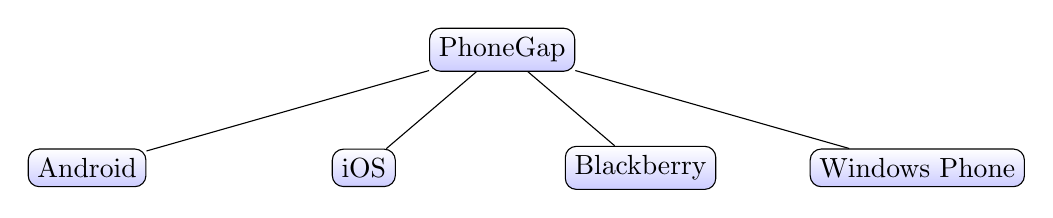
\begin{tikzpicture}[sibling distance=10em,
  every node/.style = {shape=rectangle, rounded corners,
    draw, align=center,
    top color=white, bottom color=blue!20}]]
  \node {PhoneGap}
    child { node {Android} }
    child { node {iOS} }
    child { node {Blackberry} }
    child { node {Windows Phone} };
\end{tikzpicture}
\medskip
\caption{PhoneGap can be compiled into multiple plattoforms. \label{fig:phonegap-plattforms}} 
\end{figure}

A disadvantage of developing in PhoneGap is when there is a use of many native features. The PhoneGap framework provides an API for accessing native functions when building a mobile application. Hence, if the framework is not up to date with the latest new features, the developer will not be able to partake of the features until the framework is updated. If the application is dependent on many native features a hybrid application may have limitations\cite{kohan2015}.

\subsection{Inline frame}\label{subsec:inline-frame}
In a HTML document an inline frame is used to embed another HTML within the document. The HTML document that has the inline frame is called the parent document and the HTML document that is embeded is called the child document. Communication from the parent document to the child document is easily implemented since it has direct access and can invoke JavaScript functions in the inline frame. Communicating the other way however requires more preparations. There are more than one way to solve it, one way is using the postMessage method of the parent document, and implementing a message listener.

A HTML document can be embeded in an inline frame if the HTTP response header X-Frame-Options is set to allow the embeding. There are three options the X-Frame-Options can be set to, resulting in different behavior. 
\begin{description}
 \item[DENY] \hfill \\
	The HTML document can't be displayed in an inline frame. 
\item[SAMEORIGIN] \hfill \\
	The HTML document can be displayed in an inline frame on the same origin as the HTML document. 
\item[ALLOW-FROM uri] \hfill \\
	The HTML document can only be displayed in an inline frame on the specified origin. 
\end{description}

If X-Frame-Options is removed then the HTML document can be embeded anywhere. This makes it possible to use the HTML document for malicous framing of content, called ClickJacking \cite{law2010}.

\subsection{JQuery mobile}\label{subsec:jquery-mobile}
JQuery mobile is a web or mobile application framework focused on making responsive web sites and mobile applications that are compatible with smartphones, tablets and desktop devices \cite{jquery-mobile15}. JQuery mobile is compatible with other frameworks, for example the JQuery mobile framework can be used together with the framework PhoneGap \cite{tech-republic-jquery-mobile-compatible14}. 

\subsection{Appcelerator Titanium}\label{subsec:appcelerator-titanium}
Titanium is a framework for developing mobile applications that are compatible with multiple mobile platforms such as iOS, Android, Windows Phone \cite{titanium15}. Eclipse reported 2012 that 2.8\% of mobile developers use Titanium for developing mobile applications. In Titanium the mobile application are developed from a JavaScript codebase. Titanium also allows API access to native UI components and native functionality that is not covered by Titaniums API. Developing with Titanium gives fast results but some developers have reported issues with the stability and memory management \cite{stay-away1-titanium15} \cite{stay-away2-titanium15}. 

\section{Lines of code}\label{sec:lines-of-code}
Source lines of code is a measurement tool for software development. Source lines of code, also abbreviated as SLOC, is very easy to obtain and is a fairly accurate predictor of development effort\cite[p.~63]{galorath2006}. Measuring SLOC simply means you count the number of lines of code. There are many different ways to measure SLOC, such as Halsted’s approach, function points, physical SLOC and Logical SLOC. 

Physical SLOC is the length of the code excluding comments and blanks. Function points measure functionality and can therefore be measured before the design and coding if the requirement specification is complete\cite[p.~187]{galorath2006}. Halstead’s uses measurable properties such as operands and operators and uses them to identify properties of software. Such as the length, difficulty and effort of the program. Fenton and Bieman describes Halstead’s software science measures as a confused and inadequate measurement. Particularly for other attributes then size\cite[p.~345]{fenton2015}.

Logical SLOC measures the number of statements that carry over one or more physical lines.  For languages with terminators, this can be counted more easily and quickly. As an example, in Java you could count the logical SLOC by counting the number of line-terminating semicolons and closing curly brackets. Logical SLOC represents the programming instructions and data declarations which are converted into executable instructions, i.e. the implementation of the software design. Another positive aspect of of logical SLOC is that it better handles differences in formatting and style conventions than physical SLOC\cite[p.~155]{galorath2006}.

To compare size between two different languages a size conversion table can be used. The table can be used to estimate how many SLOC a program coded in one programming language would have in another language. In the table constructed by Galorath and Evans you can compare a third generation language, a fourth generation language, Ada, Assembly or Pascal\cite[p.~163]{galorath2006}. A third generation language compared to another third generation language would have no conversion rate. 

\section{Further reading}\label{sec:further-reading}
For information and analysis about choosing the right development approach for developing a mobile application we recommend two alternatives. The first recommendation is a paper by Michaels, ross \& cole named “Native mobile apps: The wrong choice for business? ” \cite{michaels2013}. The second recommendation is an article by Kohan and Montanez named “Native vs Hybrid / PhoneGap App Development Comparison” \cite{kohan2015}. 

The paper by Michaels, ross \& cole compares the advantages and disadvantages with native applications, mobile web applications and hybrid applications. The paper analyzes aspects such as development cost and effort, maintainability and maintenance cost. 

The article by Kohan and Montanez compares native to hybrid/PhoneGap application development.  The article evaluates  limitations, development cost and user experience for the development approaches.